\section{Auswertung}
\label{sec:Auswertung}

Bevor mit der eigentlichen Messung begonnen wird, wird der Nulleffekt gemäß \autoref{sec:Durchführung} durchgeführt und die Daten in
\autoref{tab:Zerfall0} notiert.

\begin{table}[H]
  \centering
  \caption{Messdaten zur Nullmessung beim $\gamma$- und $\beta$-Zerfall.}
  \label{tab:Zerfall0}
  \sisetup{table-format=3.0}
  \begin{tabular}{S S S @{${}\pm{}$}S[table-format=2.2] S[table-format=1.2] @{${}\pm{}$}S[table-format=1.2] }
    \toprule
    \multicolumn{1}{p{2cm}} {Strahlungsart} &\multicolumn{1}{p{2cm}} {Messzeit $t / \si{\second}$} & \multicolumn{2}{c}{$N_0$}& \multicolumn{2}{c}{$\frac{N_0}{t} / \frac{1}{\si{\second}}$}\\
    \midrule
    $\gamma$ & 900 & 828 & 28.77 & 0.92 & 0.03\\
    $\beta$ & 900 & 657 & 25.63 & 0.73 & 0.03\\
  \bottomrule
  \end{tabular}
\end{table}

\subsection{Gamma-Strahlung}
\label{sub:gamma_aus}
Der Versuch wird nach \autoref{sec:Durchführung} durchgeführt und die Ergebnisse der Messungen in \autoref{tab:gammaEisen} und \autoref{tab:gammaBlei} eingetragen.
\begin{table}[H]
  \centering
  \caption{Messdaten zum $\gamma$-Zerfall mit Eisen als Absorber.}
  \label{tab:gammaEisen}
  \sisetup{table-format=2.2}
  \begin{tabular}{S[table-format=2.1] S[table-format=2.0] S[table-format=4.0]@{${}\pm{}$} S[table-format=2.2] S[table-format=3.2] @{${}\pm{}$}S[table-format=1.2]}
    \toprule
    \multicolumn{1}{p{2cm}}{ $ d/ \si{\milli\meter}$} &\multicolumn{1}{p{2cm}} {Messzeit $t / \si{\second}$} & \multicolumn{2}{c}{$N$}& \multicolumn{2}{c}{$\frac{N}{t} / \frac{1}{\si{\second}}$}\\
    \midrule
       0.0 &  60 &  6976 & 83.52 & 116.27 & 1.39 \\
       0.5 &  60 &  6738 & 82.09 & 112.30 & 1.37 \\
       1.0 &  60 &  6635 & 81.46 & 110.58 & 1.36 \\
       1.5 &  60 &  6374 & 79.84 & 106.23 & 1.33 \\
       2.0 &  60 &  6463 & 80.39 & 107.72 & 1.34 \\
       2.5 &  60 &  6261 & 79.13 & 104.35 & 1.32 \\
       3.0 &  60 &  5622 & 74.98 &  97.30 & 1.25 \\
       5.0 &  60 &  5410 & 73.55 &  90.17 & 1.23 \\
       6.0 &  60 &  5681 & 75.37 &  94.68 & 1.26 \\
       7.0 &  60 &  5318 & 72.92 &  88.63 & 1.22 \\
      10.0 &  60 &  4569 & 67.59 &  76.15 & 1.13 \\
      15.0 &  60 &  4101 & 64.04 &  68.35 & 1.07 \\
      20.0 &  60 &  2955 & 54.36 &  49.25 & 0.91 \\
      25.0 &  60 &  2428 & 49.27 &  40.47 & 0.82 \\
  \bottomrule
  \end{tabular}
\end{table}

\begin{table}[H]
  \centering
  \caption{Messdaten zum $\gamma$-Zerfall mit Blei als Absorber.}
  \label{tab:gammaBlei}
  \sisetup{table-format=2.2}
  \begin{tabular}{S[table-format=2.1] S[table-format=2.0] S[table-format=4.0]@{${}\pm{}$} S[table-format=2.2] S[table-format=3.2] @{${}\pm{}$}S[table-format=1.2]}
    \toprule
    \multicolumn{1}{p{2cm}}{ $ d/ \si{\milli\meter}$} &\multicolumn{1}{p{2cm}} {Messzeit $t / \si{\second}$} & \multicolumn{2}{c}{$N$}& \multicolumn{2}{c}{$\frac{N}{t} / \frac{1}{\si{\second}}$}\\ 
       0.0 &  60 & 6718 & 81.96 & 111.97 & 1.37 \\
       1.0 &  60 & 5866 & 76.59 &  97.77 & 1.28 \\
       2.0 &  90 & 7875 & 88.74 &  87.50 & 0.99 \\
       3.0 &  90 & 7675 & 87.61 &  85.28 & 0.97 \\
       4.0 &  90 & 6727 & 82.02 &  74.74 & 0.91 \\
       5.0 &  90 & 5963 & 77.22 &  66.26 & 0.86 \\
       6.0 &  90 & 5287 & 72.71 &  58.74 & 0.81 \\
      10.0 & 120 & 5014 & 70.81 &  41.78 & 0.59 \\
      11.0 & 150 & 5913 & 76.90 &  39.42 & 0.51 \\
      12.0 & 150 & 5363 & 73.23 &  35.75 & 0.49 \\
      14.0 & 180 & 5103 & 71.44 &  28.35 & 0.40 \\
      15.0 & 180 & 4511 & 67.16 &  25.06 & 0.37 \\
  \bottomrule
  \end{tabular}
\end{table}

Aus den Messwerten wird die Aktivität 
\begin{align}
  A= \frac{N}{t}-\frac{N_0}{t}
\end{align}
berechnet.
Diese wird logarithmisch in Beziehung zur Schichtdicke $d$ in \autoref{fig:plot1} beziehungsweise \autoref{fig:plot2} dargestellt.
Außerdem wird mithilfe vom Pythonmodul matplotlib \cite{matplotlib} eine lineare Regression der Form $a \cdot x + b$ berechnet und 
als Ausgleichsgerade in den Plot eingetragen.

\begin{figure}[H]
  \begin{subfigure}{\textwidth}
    \centering
    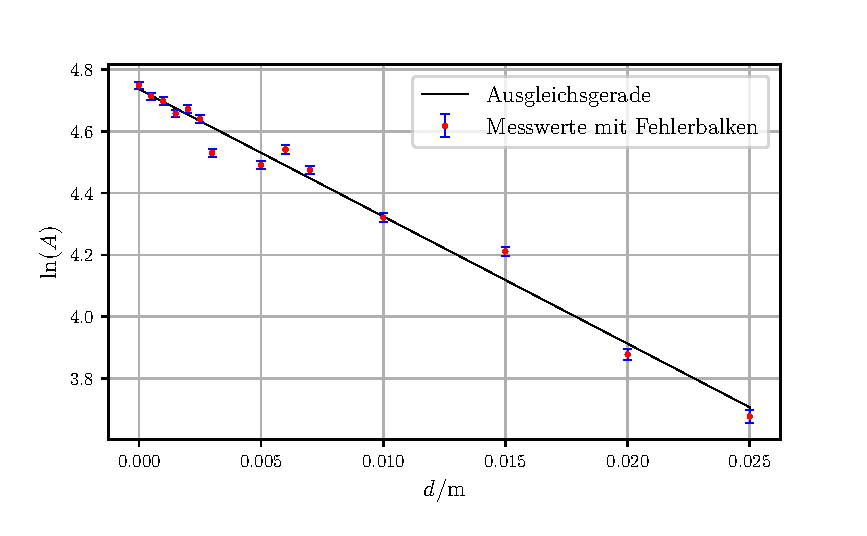
\includegraphics[scale=0.75]{build/plot1.pdf}
    \caption {Lineare Ausgleichsrechung zur Bestimmung des Absorptionskoeffizienten
    $\mu_{\text{Fe}}$ von Eisen.}
    \label{fig:plot1}
  \end{subfigure}
  \hfill
  \begin{subfigure}{\textwidth}
    \centering
    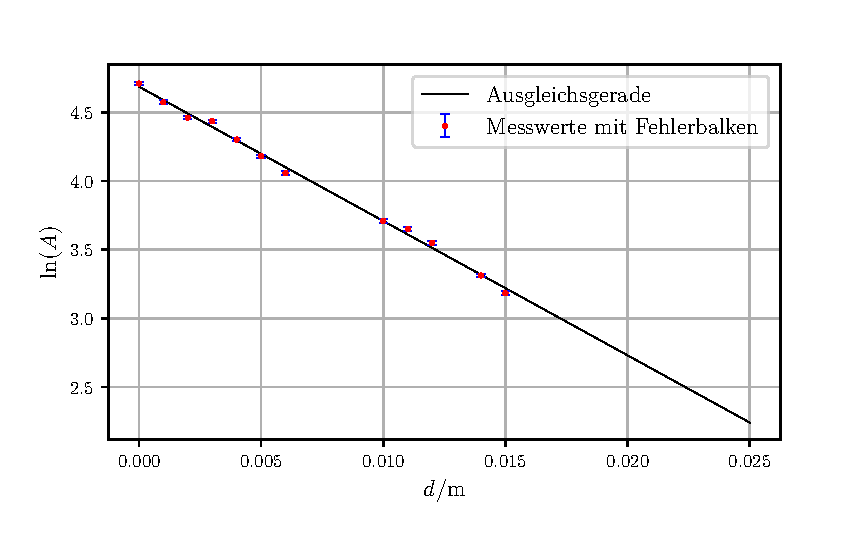
\includegraphics[scale=0.75]{build/plot2.pdf}
    \caption {Lineare Ausgleichsrechung zur Bestimmung des Absorptionskoeffizienten
    $\mu_{\text{Pb}}$ von Blei.}
    \label{fig:plot2}
  \end{subfigure}
    \caption {Messdaten zur Bestimmung der Absorptionskoeffizienten aus der Zählrate.}
  \end{figure}

Der Absorptionskoeffizient entspricht der negativen Steigung der Geraden
\begin{align*}
  -a_{\text{Fe}} &= &\mu_{\text{Fe}} &= & (41.16 \pm 1.56) \si{\per\meter}\\
  -a_{\text{Pb}} &= &\mu_{\text{Pb}} &= & (97.80 \pm 1.81) \si{\per\meter}.
\end{align*}
Dies Größe $N(0)$ wird jeweils als erstes durch eine Messung ohne eingesetze Absorber bestimmt und ist in \autoref{tab:gammaEisen}
und \autoref{tab:gammaBlei} aufgeführt.

\subsection{Beta-Strahlung}
\label{sub:beta_aus}
Die Messung wird wie in \autoref{sec:Durchführung} durchgeführt und die Werte werden in \autoref{tab:beta} aufgetragen. 
Außerdem ist in der Tabelle auch der Nulleffekt $A_U$ pro Zeit (siehe \autoref{tab:Zerfall0}) von der AKtivität $A$ pro Zeit abgezogen.

\begin{table}[H]
  \centering
  \caption{Messdaten von $\beta$-Strahlung durch Aluminium.}
  \label{tab:beta}
  \sisetup{table-format=2.2}
  \begin{tabular}{S[table-format=3.0] S[table-format=3.0] S[table-format=5.0] @{${}\pm{}$} S[table-format=3.2] S[table-format=3.2] @{${}\pm{}$} S[table-format=2.2]}
  \toprule
  {Dicke $d / \si{\micro\meter}$} & {Zeit $t / \si{\second}$} & \multicolumn{2}{c}{$N$} & \multicolumn{2}{c}{$\; \; A-A_U \, / \, \frac{1}{\si{\second}}$} \\
  \midrule
      0   &   100 &   57621   &   240 &   575.54  &   2.37   \\
      100 &   100 &   4093    &   64  &   40.20   &   0.61    \\
      125 &   100 &   973     &   31  &   9.00    &   0.28    \\
      153 &   150 &   1537    &   39  &   9.52    &   0.23    \\
      160 &   150 &   897     &   30  &   5.25    &   0.17    \\
      200 &   200 &   456     &   21  &   1.55    &   0.08    \\
      253 &   300 &   207     &   14  &   -0.04   &   0.02    \\
      302 &   300 &   208     &   14  &   -0.04   &   0.02    \\
      338 &   300 &   225     &   15  &   0.02    &   0.02    \\
      400 &   400 &   280     &   17  &   -0.03   &   0.01    \\
      444 &   450 &   593     &   24  &   0.59    &   0.03    \\
      482 &   450 &   319     &   18  &   -0.02   &   0.01    \\
  \bottomrule
  \end{tabular}
\end{table}


 Die Aktivität $A-A_U$ wird logarithmisch in Beziehung zur Schichtdicke $d$ in \autoref{fig:plot3}.
\begin{figure}[H]
  \centering
  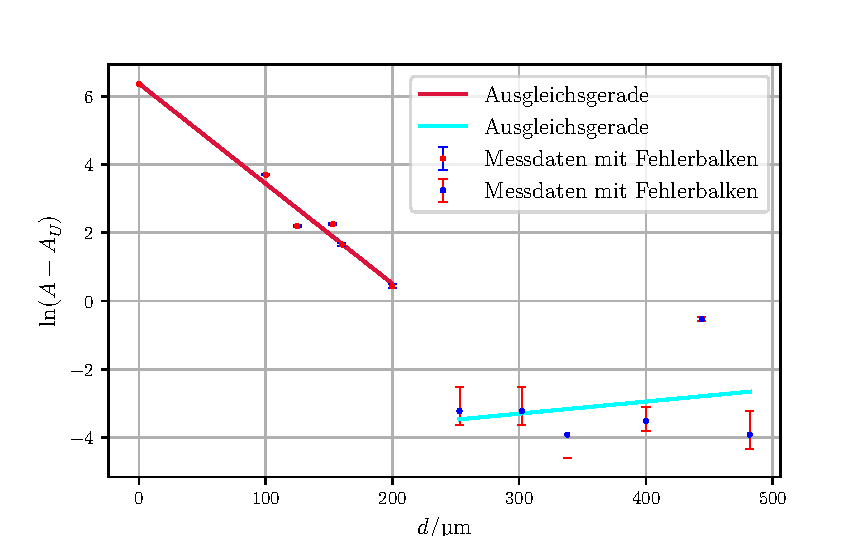
\includegraphics{build/plot3.pdf}
  \caption {Lineare Regression der Aktivität aufgetragen gegen die Dicke.}
  \label{fig:plot3}
\end{figure}

Auch hier wird mithilfe vom Pythonmodul matplotlib \cite{matplotlib} eine lineare Regression der Form $a \cdot x + b$ berechnet und 
als Ausgleichsgerade in den Plot eingetragen. 
Die Werte der Koeffizienten der Ausgleichsgrade werden zu
\begin{align*}
  a_1 &= (-0.029 \pm 0.002) \frac{1}{\si{\micro\meter}}\\
  b_1 &= (6.372 \pm 0.305) \\
  a_2 &= (0.004 \pm 0.007) \frac{1}{\si{\micro\meter}}\\
  b_2 &= (-4.357 \pm 2.673)
\end{align*}
berechnet.
Die x-Koordinate des Schnittpunkts der beiden Ausgleichsgeraden ist der Wert $R_{max}$ und ergibt
sich aus
\begin{equation}
  R_{max} =  \frac{b_2 - b_1}{a_1 - a_2}
  \label{eqn:Rmax}
\end{equation}
dieser muss dann noch mit der Dichte von Aluminium $\rho = 2700 \frac{kg}{m^3}$\cite{AlDichte} und ergibt sich somit zu
\begin{align}
  R_{max} &= 0,878 \frac{\si{kg}{\meter^2}}.
\end{align}

Der Fehler von $R_{max}$ wird mit der Gauß'schen Fehlerfortpflanzung 
\begin{align*}
  \sigma_R = \sqrt{
      \sum\limits_{i = 1}^N
       \left( \frac{\partial f}{\partial x_i} \sigma_i \right)^{\!\! 2}
     }
     =\sqrt{\frac{\sigma_{a_{1}}^{2} \left(- b_{1} + b_{2}\right)^{2}}{\left(- a_{1} + a_{2}\right)^{4}}
  + \frac{\sigma_{a_{2}}^{2} \left(- b_{1} + b_{2}\right)^{2}}{\left(- a_{1} + a_{2}\right)^{4}} + \frac{\sigma_{b_{1}}^{2}}{\left(- a_{1}
  + a_{2}\right)^{2}} + \frac{\sigma_{b_{2}}^{2}}{\left(- a_{1} + a_{2}\right)^{2}}}
\end{align*}
berechnet, sodass sich $R_max$ zu
\begin{align}
  R_{max}= (325.121 \pm 81,56) \si{\micro\meter}
\end{align}
ergibt. Damit und mit \autoref{eqn:Emax} kann die Energie $E_{max}$ zu
\begin{align}
  E_{max}= 624,443 \si{}.
\end{align}
